\section{\seccountingsubsets}
\label{sec_counting_subsets}

In \Cref{sec_counting_steps_cases} we counted strings and other ordered objects.  How might we count the number of ways to choose some items from a set when we do not care about the order, like a group of students to work on a project? In this section, we discuss subsets and introduce the binomial coefficients that count subsets.  We combine counting subsets with our other rules for counting: steps (\Cref{thm_steps_multiply}), cases (\Cref{thm_cases_add}), and counting the opposite (\Cref{thm_count_complement}). We also introduce our first proof format, which is for combinatorial proof.

Before we learn any new rules, try the following activity.

\begin{act} [Adopting two cats]
\label{act_adopting_two_cats}  
~
    \begin{actpart}
        \item \label{part_list_two_cats} There are five cats (\str{c1}, \str{c2}, \str{c3}, \str{c4}, \str{c5}) waiting to be adopted at the animal shelter. You want to adopt two of the cats.  Make a list of possibilities. Notice that the order in which we choose the cats does not matter.  For example, choosing \str{c2} and \str{c5} is the same as choosing \str{c5} and \str{c2}.  For that reason, we use set notation to indicate a choice, such as $\{\str{c2}, \str{c5}\}$.
        \item \label{part_choose_two_cats} In how many ways can you choose two cats to adopt?
        \item Betelehem tried to answer (\ref{part_choose_two_cats}) without making a list. Here is her work.
            \begin{soln}
                We will count the possibilities using steps.
            
                Step 1: Choose the first cat. (5 ways)

                Step 2: Choose the second cat.  Note that the second cat must be a different cat from the first cat. (4 ways)

                Since steps multiply (\Cref{thm_steps_multiply}), there must be $5 \times 4 = 20$ ways to adopt two cats.        
            \end{soln}

        Uh oh!  The correct answer is ten, so Betelehem's answer is incorrect. (Hint: If you also had 20, you should go back and fix your work.) What went wrong?  Explain.  Hint: Betelehem's answer is exactly twice ($\times 2$) the correct answer, so she must have \vocab{double counted} (counted each pair twice). 
        \item \label{part_kchoose2_cats} If there were $k$ cats and you wanted to adopt two cats, how many possibilities are there?  Hint: You can use Betelehem's approach as long as you remember that you will get twice the correct answer.  Another hint: handshakes! 
    \end{actpart}
\end{act} 

%%%%%%%%%%%%%%%%%%%%%%%%%%%%%%%%%%%%%%%%%%%%%%%%%%%%%%%%%
\newcommand{\subsubsetschoose}{Subsets and the Binomial Coefficients}
\subsection{\subsubsetschoose}
\label{sub_subsets_choose}

In many situations, we want to select some of the elements of a set.  We can think of a set as corralling\footnote{The word \vocab{corral} means to collect and contain.  A common usage is in reference to fencing in animals such as horses or sheep.} its elements inside a rope.  For example, the set $A=\{1,2,3,7,8\}$ is drawn in \Cref{fig_subset_corral}.  If we corral some, all, or none of the elements within $A$, we get a subset of $A$.  For example, \Cref{fig_subset_corral} shows the subset $\{2,8\}$ shaded in gray.

\begin{figure}[ht]
    \centering
        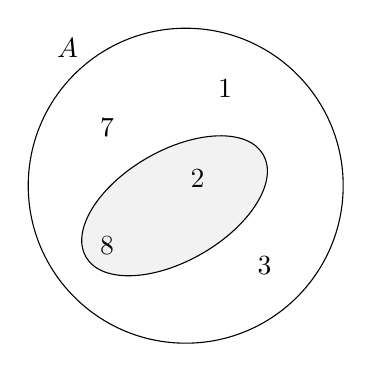
\begin{tikzpicture}[set/.style={fill=gray,fill opacity=0.1}]
            \scope
            \clip 
            (0,0) circle (1);
            \endscope
    \draw (0,0) circle (2) 
        (-1.5,1.5) node [text=black,above] {$A$}
          (.5,1)node [text=black,above] {$1$}
            (.15,-.15)node [text=black,above] {$2$}
              (1,-1.25)node [text=black,above] {$3$}
                (-1,.5)node [text=black,above] {$7$}
                  (-1,-1)node [text=black,above] {$8$}
                      %(1,.5) node [text=black,above] {$B$}
    ;
    \draw[set,rotate =30] (-.25,-.15) ellipse (1.3cm and .7cm);
    \end{tikzpicture}
    \caption{The subset $\{2,8\}$ corrals some of the elements of the set $A=\{1,2,3,7,8\}$.}
        \label{fig_subset_corral}
\end{figure}

We formally define a subset.

\begin{defn}[Subsets]
\label{defn_subsets}
~
    \begin{apart}
        \item A \vocab{subset} of the set $A$ is a set consisting of some of the elements of $A$, where the word ``some'' is understood to be any number of elements-- from none to all. That is, the set $T$ is a subset of the set $A$, denoted $T \subseteq A$ if every element of $T$ is also an element of $A$.  For example, $\{2,8\} \subseteq \{1,2,3,7,8\}$ and $\{3\} \subseteq \{1,2,3,7,8\}$. Note that the set $A$ is a subset of itself.  For example, $\{1,2,3,7,8\} \subseteq \{1,2,3,7,8\}$.
        
        \item The \textbf{empty set} $\varnothing$ is the set with no elements. That is $\varnothing=\{ ~\}$. 
        Note that $\varnothing$ is a subset of any set. Imagine corralling no elements or drawing a shaded shape within $A$ that contains none of the elements of $A$. For example, $\varnothing \subseteq \{1,2,3,7,8\}$.  
    \end{apart}
\end{defn}

\begin{rem}[Notation for zero]
\label{rem_notation_zero}
   Computer scientists often write the number zero with a slash to avoid confusion with the letter $O$, so the zero symbol in computer science looks similar to the empty set symbol $\varnothing$.  In this textbook, we write $0$ for zero without a slash and save $\varnothing$ to mean the empty set.
   %%SU I can't figure out how to typeset the zero-slash symbol without messing up texttt in general
\end{rem} 

In \Cref{act_adopting_two_cats}, we chose two cats from a set of five cats. It is useful to have a name for the number of ways to select exactly $k$ objects from a set of $n$ distinct objects.  

\begin{defn} [Binomial coefficient]
\label{defn_binomial_coeff}
    For non-negative integers $k$ and $n$,
    \begin{apart}
        \item The number of ways to select a subset of $k$ elements from a set of $n$ elements is the \vocab{binomial coefficient}
        $\binom{n}{k}$
        which is pronounced ``$n$ choose $k$.''  For example, ``5 choose 2'' is $\binom{5}{2} = 10$
        because we saw in \Cref{act_adopting_two_cats} that there are 10 ways to select two cats from a set of five cats. 
        \item Note that if $k>n$, then $\binom{n}{k}=0$.
    \end{apart}
\end{defn}

The simplest way to evaluate a binomial coefficient is to search for it on the Internet or ask a virtual assistant. For example, search for ``five choose two'' and you will get ten. You can also evaluate binomial coefficients using some calculators and spreadsheet programs.
Therefore, it is perfectly acceptable to leave binomial coefficients in an answer to a counting problem.

\begin{rem} [Not evaluating counts, version 3]
\label{rem_not_eval_counts_3}
Unless stated otherwise, when counting you may leave any answer greater than twenty in a format that could easily be evaluated on a calculator. In particular, your answer may involve addition, subtraction, multiplication, division, factorials, binomial coefficients, and parentheses.
\end{rem}

For small values, we can evaluate binomial coefficients by listing the possible subsets.  As usual, working with small values can help us to understand the concept.

\begin{exam}[Four choose $k$]
\label{exam_four_choose_k}
Evaluate $\binom{4}{k}$ for each nonnegative integer $k$ by listing the $k$-element subsets of $\{1,2,3,4\}$.
    \begin{soln}
        When $k=0$, the only 0-element subset is $\varnothing$ and so $\binom{4}{0}=1.$

        When $k=1$, the 1-element subsets are
        $\{1\}, \{2\}, \{3\}, \{4\}$ and so $\binom{4}{1}=4.$

        When $k=2$, the 2-element subsets are 
        $\{1,2\}, \{1,3\}, \{1,4\}, \{2,3\}, \{2,4\}, \{3,4\}$
        and so $\binom{4}{2}=6.$
        
        When $k=3$, the 3-element subsets are 
        $\{1,2,3\}, \{1,2,4\}, \{1,3, 4\}, \{2,3,4\}$
        and so $\binom{4}{3}=4.$

        When $k=4$, the only 4-element subset is
        $\{1,2,3,4\}$
        and so $\binom{4}{4}=1.$

        When $k >4$ we have 
        $\binom{4}{k}=0 \text{ for } k>4.$
    \end{soln}
\end{exam}

It is your turn to use subsets to evaluate some small binomial coefficients.

\begin{act} [Six choose $k$]
\label{act_eval_6choosek}
~    
    \begin{actpart}
        \item Evaluate $\binom{6}{0}$, $\binom{6}{1}$, and $\binom{6}{6}$ by listing subsets of $\{1,2,\ldots,6\}$.
        \item Conjecture the values of $\binom{n}{0}$, $\binom{n}{1}$, and $\binom{n}{n}$ where $n$ is a positive integer.
        \item Evaluate $\binom{6}{5}$ by listing subsets of $\{1,2,\ldots,6\}$.  Hint: stay organized by considering which integer is not in the set.
        \item Conjecture the value of $\binom{n}{n-1}$ where $n$ is a positive integer.
    \end{actpart}
\end{act}

%%%%%%%%%%%%%%%%%%%%%%%%%%%%%%%%%%%%%%%%%%%%%%%%%%%%%%%%%
\newcommand{\subcombinecount}{Combining Counting Techniques}
\subsection{\subcombinecount}
\label{sub_combine_count}

Many counting problems require a combination of techniques we have learned, including cases, steps, opposites, and subsets.  

\begin{exam}[Team and leader]
\label{exam_team_leader}   
    There are 25 students in the coding club, ten of whom are first-year students.  For the coding competition, we need a team of four students that includes exactly one first-year student.  How many different teams are possible?
    \begin{soln}
        Since ten of the 25 students are first-year students, the other $25-10=15$ are not first-year students.  To make a team of four with exactly one first-year student, we will also need three students who are not first-year.

        Step 1: Choose the first-year student.  We want one first-year student out of ten, so there are $\binom{10}{1} = 10$ ways to do this step.

        Step 2: Choose the other three students.  We want three students who are not first year out of 15, so there are $\binom{15}{3}$ ways to do this step.

        Since steps multiply (\Cref{thm_steps_multiply}), there are a total of 
        $$\binom{10}{1}\binom{15}{3} = 10\binom{15}{3} = \text{4,550}$$
        ways to choose a team.        
    \end{soln}
\end{exam}

Try your hand at combining these techniques. 

\begin{act} [Adopting two animals]
\label{act_adopting_two_animals}  
There are five cats and 12 dogs waiting to be adopted.
    \begin{actpart}
        \item \label{part_two_animals} In how many ways can you choose two animals to adopt?  Hint: How many animals are there?
        \item \label{part_two_cats} In how many ways can you choose two animals to adopt if they are both cats? Write your answer as a binomial coefficient.  (Yes, we made a list and counted this same number in \Cref{act_adopting_two_cats}).
        \item \label{part_two_dogs} In how many ways can you choose two animals to adopt if they are both dogs?
        \item \label{part_cat_dog} In how many ways can you choose two animals to adopt if you choose one cat and one dog?
        \item How are your answers to (\ref{part_two_cats}), (\ref{part_two_dogs}), and (\ref{part_cat_dog}) related to your answer to (\ref{part_two_animals})?  Use technology to evaluate the binomial coefficients.
        \item Why?  Hint: Use cases. \end{actpart}
\end{act}

Several exercises in this section refer to a 52-card deck of playing cards, shown in \Cref{fig_52card_deck}.  The key facts to know are stated in the following definition.

\begin{defn}[52-card deck of playing cards]
\label{defn_52-card_deck}
~
    \begin{apart}
        \item A \vocab{hand} is a set of cards, without regard to order.  The name comes from the fact that in many card games you hold the cards in your hand. The number of cards in a hand varies depending on the game.  Poker is a family of card games that often uses hands with five or seven cards, whereas Bridge is a card game that uses hands with thirteen cards.
        \item Each card in the deck has one of thirteen \vocab{denominations}:  
        \begin{center} 
        Ace (A), 2, 3, 4, 5, 6, 7, 8, 9, 10, Jack (J), Queen (Q), or King (K).  
        \end{center}
        \item Each card in the deck also has one of four \vocab{suits}
        \begin{center} 
        clubs $\clubsuit$, diamonds $\diamondsuit$, hearts $\heartsuit$, or spades $\spadesuit$.
        \end{center}
        For example, a card might be the Jack of hearts, denoted J$\heartsuit$.  
        Note that for each choice of denomination and suit, there is exactly one card with that denomination and suit.  For example, there is exactly one card that is J$\heartsuit$.
        \item The cards with clubs and spades are \vocab{black cards}.  The cards with diamonds and hearts are \vocab{red cards}.
    \end{apart}  
\end{defn} 

    \begin{figure}[ht]
        \centering
        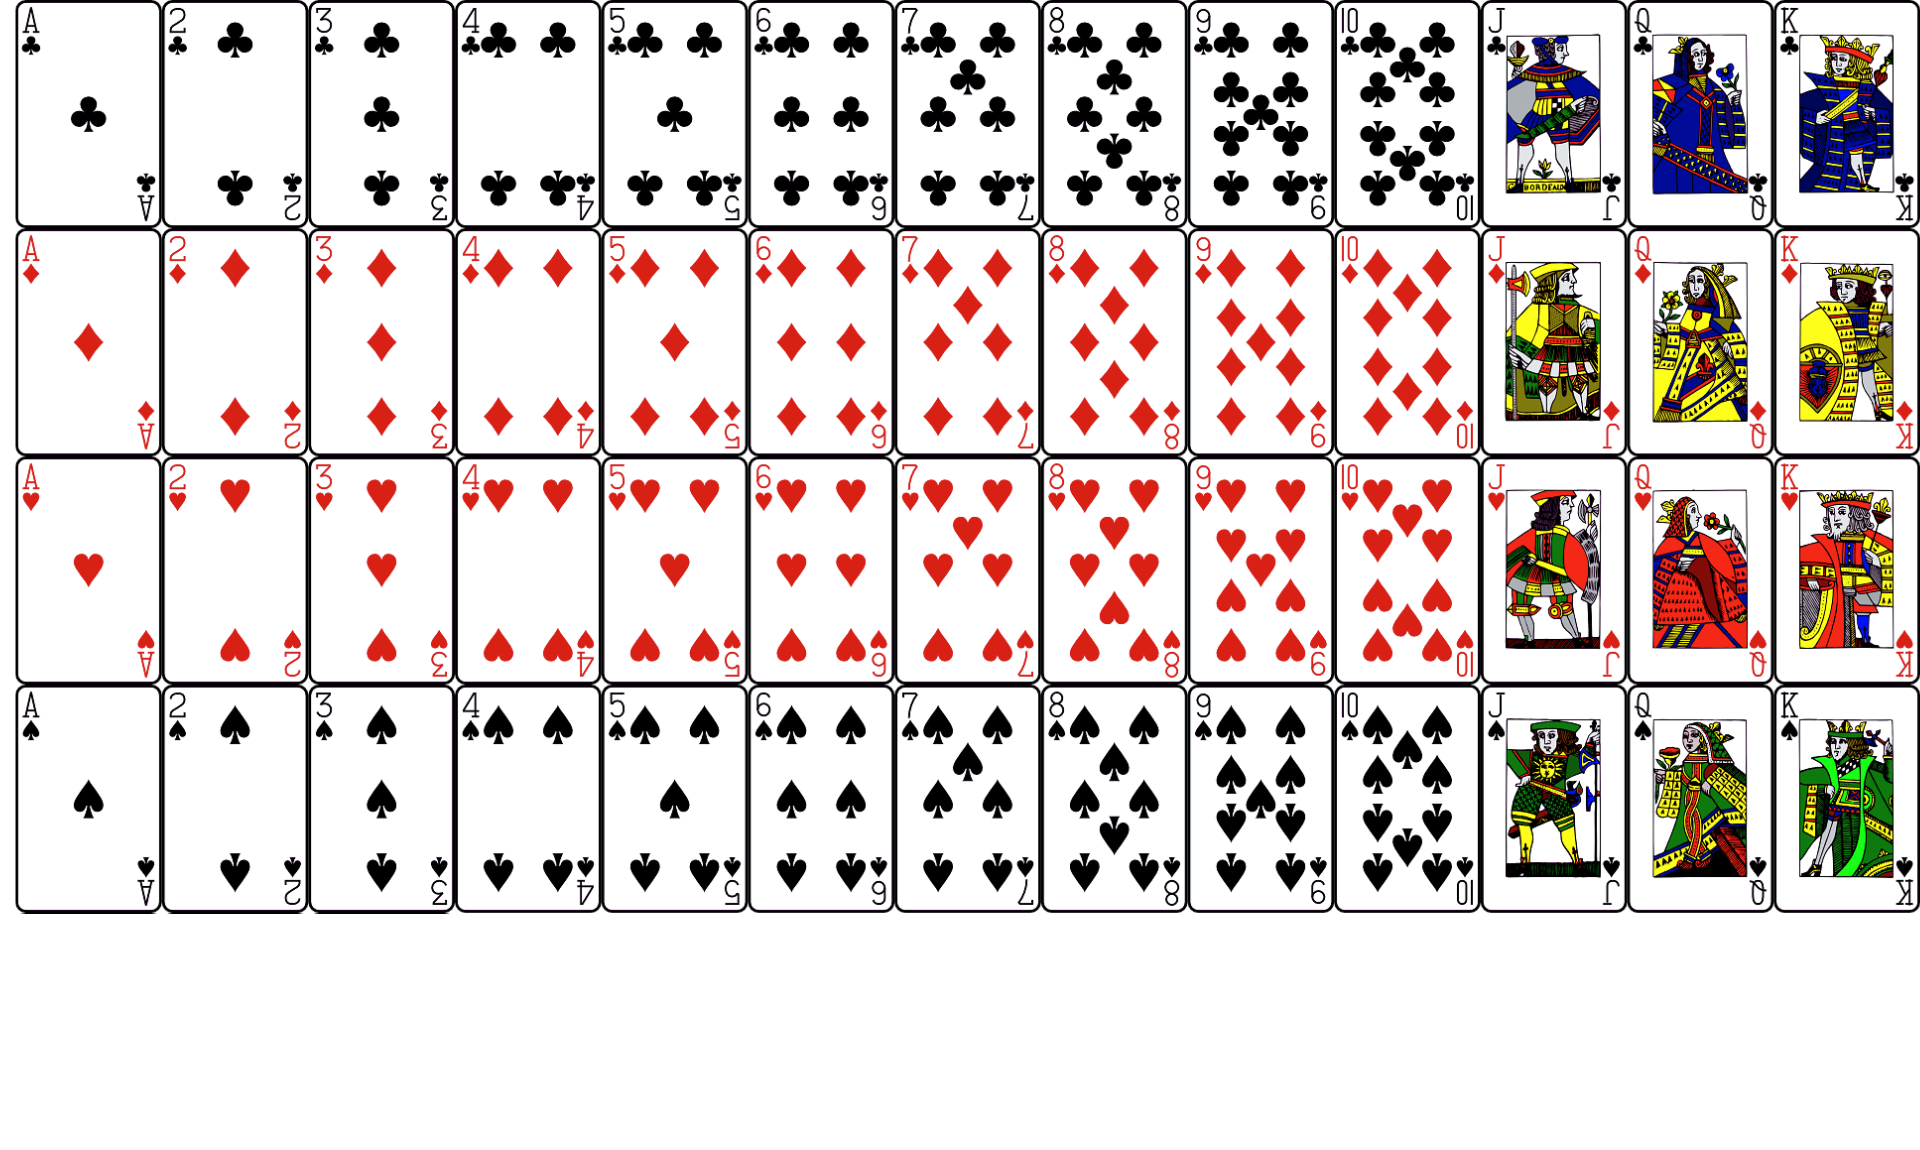
\includegraphics[width= .75\textwidth]{Images/52-card_deck_Pixabay.png}
        \caption{A 52-card deck of playing cards (source: Pixabay).}
        \label{fig_52card_deck}
    \end{figure}

Here is an example of counting hands.

\begin{exam} [Three-of-a-kind]
\label{exam_4ofakind}
    In a 52-card deck of playing cards, as shown in \Cref{fig_52card_deck}, how many 5-card hands have a \vocab{three-of-a-kind}, which is three cards of one denomination, a fourth card of a different denomination, and fifth card of another denomination.\footnote{The fourth or fifth cards cannot be the same denomination as the three-of-a-kind because that is a \vocab{four-of-a-kind}.  The fourth and fifth cards cannot be the same denomination as each other because that is a \vocab{full house}.}  
    How many different 5-card hands have a three-of-a-kind?
    \begin{soln}
        Let's build such a hand through a series of steps.

        Step 1: Select the denomination of the three-of-a-kind.  Since there are 13 denominations, there are $\binom{13}{1} = 13$ ways to complete this step.

        Step 2: Select the cards for the three-of-a-kind.  There are four cards in the denomination we chose in Step 1 and we want three of them, so there are $\binom{4}{3} = 4$ ways to complete this step.

        Step 3: Select the denominations of the other two cards.  Since there are $13-1=12$ remaining denominations and we want two of them, there are $\binom{12}{2}$ ways to complete this step.  

        Step 4: Select the cards in the other two denominations.  Since there are four cards in each denomination chosen in Step 3, there are $\binom{4}{1}$ ways to choose each. Since there are two cards and steps multiply (\Cref{thm_steps_multiply}), there are $\binom{4}{1}\binom{4}{1} = 4 \times 4 = 16$ ways to complete this step, which finishes building our hand.

        Since steps multiply (\Cref{thm_steps_multiply}), there are 
        $$\binom{13}{1}\binom{4}{3}\binom{13}{2}\binom{4}{1}\binom{4}{1} = (13)(4)\binom{13}{2}(4)(4) =4^3(13)\binom{12}{2}=\text{64,896}$$
        ways. (Any of those formats of the answer is acceptable.)
    \end{soln}
\end{exam}

%%%%%%%%%%%%%%%%%%%%%%%%%%%%%%%%%%%%%%%%%%%

\newcommand{\subproofscountnosums}{Proof Format: Combinatorial Proof}
\subsection{\subproofscountnosums}
\label{sub_proofs_count_nosums}

Jarrett and Xueqing solve the same counting problem, but they use two different methods.  They should still get the same answer, right?  This observation can lead to a way to prove that two quantities are equal: Jarrett's answer = Xueqing's answer.  This strategy might remind you of the saying ``six of one, half dozen of the other'' which sounds like two different quantities, but because a dozen is twelve, half a dozen is also six.

There are many different types of proof. A \vocab{proof format} is a structure or outline of a particular type of proof.  Our first proof format is \vocab{combinatorial proof}, a \vocab{proof that counts}, in which we prove that two quantities are equal by counting the same situation using two different methods.

\begin{pff} [Combinatorial proof]
\label{pff_comb_proof} 
Prove: $N=M$ using a combinatorial proof.
    \begin{proof}
        We use a combinatorial proof. Consider the following situation \ldots. 
  
        How many ways are there to \ldots? 
        
        First, (explain how to count using one method to get $N$.) 
        
        On the other hand, (explain how to count using a different method to get $M$.) 
        
        Since we counted the same quantity in two different ways, it follows that $N=M$.  
\end{proof}
\end{pff}

Whenever we introduce a new proof format, we present an example of such a proof and then ask you to write a very similar proof by copying the example proof \emph{mutatis mutandis (mm)}, which means changing what needs to be changed. 

\begin{act}[Combinatorial proof -- choosing two animals]
\label{act_comb_proof_two_animals} 
~
    \begin{actpart}
        \item \label{part_comb_proof_read} Copy the following example of a combinatorial proof. Yes, that means copy every word.
        
        Use a combinatorial proof to prove for any positive integers $m$ and $n$ that $$\binom{m+n}{2} = \binom{m}{2} + \binom{n}{2} + mn$$
        
        \emph{Proof}  We use a combinatorial proof.  Consider the following situation: there are $m$ cats and $n$ dogs and we want to adopt two animals.  How many ways are there to choose the two animals?
            
        First, since there are a total of $m+n$ animals and we want to choose two of them, the answer is $\binom{m+n}{2}.$
            
        On the other hand, we can consider three cases.

        Case 1: Choose two cats.  In this case, we want two out of $m$ cats, and so there are $\binom{m}{2}$ ways to choose the two animals.
            
        Case 2: Choose two dogs.  In this case, we want two out of $n$ dogs, and so there are $\binom{n}{2}$ ways to choose the two animals.
            
        Case 3: The only remaining case is that we choose one cat and one dog.  In this case, we want one out of $m$ cats ($m$ ways) and then one out of $n$ dogs ($n$ ways).  Since steps multiply (by \Cref{thm_steps_multiply}), there are $mn$ ways to choose the two animals.
            
        Since cases add (by \Cref{thm_cases_add}), there is a total of $\binom{m}{2} + \binom{n}{2} + mn$ ways to choose two animals.
            
        Since we counted the same quantity in two different ways, it follows that $\binom{m+n}{2} =\binom{m}{2} + \binom{n}{2} + mn$
        
        \item Edit the proof you copied in (\ref{part_comb_proof_read}), changing what needs to be changed to prove for any positive integer $n$ that $$\binom{2n}{2} = 2\binom{n}{2} + n^2.$$
        
    \end{actpart}   
\end{act}

Here is another example of a combinatorial proof.

\begin{exam} [Combinatorial proof -- team and leader]
\label{exam_comb_proof_teamandleader}
    Use a combinatorial proof to prove that 
    $$\displaystyle 7\binom{10}{7} = 10 \binom{9}{6}$$

    \begin{soln}
    ~
        \emph{Proof.} We use a combinatorial proof.  Consider the following situation: there is a group of ten employees.  How many ways are there to choose seven employees to be on a project team where one member of the team is the project leader?

        First, we can choose the seven-person project team from the group of ten employees.  There are $\binom{10}{7}$ ways to do this step.  Then we need to choose one of those seven people on the project team to be the project leader.  There are seven ways to do this step. (You could think of it as $\binom{7}{1}$ ways, but $\binom{7}{1}= 7$ and that is simpler.)  Since steps multiply (\Cref{thm_steps_multiply}), the answer is $7\binom{10}{7}$. 

        On the other hand, we can make the choices in reverse order.  We can start by choosing the project leader, one of the ten people.  There are ten ways to do this step.  Then we need to choose the rest of the project team.  Since we already chose the project leader, we only need six more people out of the nine remaining people.  There are $\binom{9}{6}$ ways to do this step.  Since steps multiply (\Cref{thm_steps_multiply}), the answer is also $10 \binom{9}{6}$.

        Since we counted the same quantity in two different ways, it follows that $7\binom{10}{7} = 10\binom{9}{6}$. \hfill 
    \end{soln}
\end{exam}

In \Cref{act_eval_6choosek} we calculated $\binom{6}{0}=\binom{6}{6}=1$ and $\binom{6}{1}=\binom{6}{5}=6$.  We conjectured that for any integer $n$ we have$ \binom{n}{0}=\binom{n}{n}=1$ and $\binom{n}{1}=\binom{n}{n-1}=n$. In the next proof, we use a combinatorial proof to show the symmetry of the binomial coefficients, in general.

\begin{thm}[Symmetry of the binomial coefficients]
\label{thm_sym_binom}
    For any positive integers $n$ and $k$ we have
    $$\binom{n}{k}=\binom{n}{n-k}.$$
\end{thm}

Let's look at a combinatorial proof of this theorem.

\begin{exam}[Combinatorial proof -- symmetry of the binomial coefficients]
\label{exam_comb_pf_sym_arith_tri}
     Give a combinatorial proof of \Cref{thm_sym_binom}.
            \begin{soln}
                \emph{Proof}  We use a combinatorial proof.  Consider the following situation: there are $n$ people who auditioned for a play, and we want to choose $k$ people to be in the play. How many ways are there to do this?

                First, since we want to choose $k$ out of $n$ people, there are $\binom{n}{k}$ ways to select who is in the play. 

                On the other hand, instead of deciding who will be in the play, we can choose which people will not be in the play.  There are $n-k$ people who auditioned but will not be in the play, so there are $\binom{n}{n-k}$ ways to select who will be in the play in this way.

                Since we counted the same quantity in two different ways, it follows that $\binom{n}{k} = \binom{n}{n-k}.$
            \end{soln}
\end{exam}

%%%%%%%%%%%%%%%%%%%%%%%%%%%%%%%%%%%%%

\subsection{Exercises}

%%%%%%%%%%%%%%%%%%%%%%%%%%%%%%%%%%%%%%%%%%%%%%

\subsubsection*{Exercises for \Cref{sub_subsets_choose} \subsubsetschoose}

\begin{exer} [\exerP] % evaluating binomial coefficients by listing subsets]
\label{exer_eval_binomial_coeffs_list_subsets}
~
    \begin{exerpart}
        \item Evaluate $\binom{3}{k}$ for $k = 0, 1, 2, 3$ by listing the subsets of $\{1,2,3\}$.
        \item Evaluate $\binom{2}{k}$ for $k = 0, 1, 2$ by listing the subsets of $\{1,2\}$.
        \item Evaluate $\binom{1}{k}$ for $k = 0, 1$ by listing the subsets of $\{1\}$.
        \item Evaluate $\binom{0}{k}$ for $k = 0$ by listing the subsets of $\varnothing$.
    \end{exerpart}
\end{exer}

\begin{exer} [\exerP] % course selection]
\label{exer_course_selection}
There are five courses that I would like to take this semester: Architectural drawing (A), bioinformatics (B), computational theory (C), differential equations (D), and ecological models (E).
    \begin{exerpart}
        \item If I can take three of these courses, what are my options?  List them.
        \item If I can take four of these courses, what are my options?  List them.
        \item Based on your answers, evaluate $\binom{5}{3}$ and $ \binom{5}{4}$ and check your answers using technology.
    \end{exerpart}
\end{exer}

\begin{exer}[\exerP] % choosing books to read
\label{exer_library_books}
    The library's new arrivals section offers 24 mystery novels, 50 young adult novels, 17 biographies, and 46 fantasy novels. In each part of this problem, your answer should be a binomial coefficient.
        \begin{exerpart}
            \item In how many ways can I choose two young adult novels for my niece? 
            \item In how many ways can I choose three mystery novels to take on vacation?
            \item My brother likes to read biographies, but he also likes fantasy novels.  In how many ways can I choose four books to bring him?
        \end{exerpart}
\end{exer}

\begin{exer} [\exerU] % evaluating edge values of binomial coefficients]
\label{exer_eval_edge_binomial_coeffs}
    Explain how to evaluate each quantity involving a positive integer $n$ by explicitly discussing the subsets of $S = \{1,2,3,4,\ldots, n\}$.  
        \begin{exerpart}
            \item $\binom{n}{0}$
            \item $\binom{n}{1}$
            \item $\binom{n}{n}$
        \end{exerpart}
\end{exer}

\begin{exer}[\exerR] % subsets and the binomial coeffs
\label{exer_dyk_binomial_coeffs}
    Do you know \ldots
        \begin{exerpart}
            \item How to pronounce $\binom{n}{k}$?
            \item What $\binom{n}{k}$ counts?
            \item How to evaluate $\binom{n}{k}$ for small values of $n$ by listing subsets?      
        \end{exerpart}
\end{exer}

%%%%%%%%%%%%%%%%%%%%%%%%%%%%%%
\subsubsection*{Exercises for \Cref{sub_combine_count} \subcombinecount}

\begin{exer} [\exerP] % 5-card hands]
\label{exer_5card_hands}
This problem refers to the 52-card deck of playing cards in \Cref{defn_52-card_deck}.
    \begin{exerpart}
        \item How many different ways are there to deal a hand of five cards?  
        \item How many different hands have all five cards of the same suit?  Hint: First choose one of the four suits and then choose the cards.  There are 13 cards in each suit.
    \end{exerpart}
\end{exer}

\begin{exer}[\exerP] % volleyball tryouts
\label{exer_volleyball}
  There are usually 16 players on a Division III volleyball team.  Of those, six players are starters, which means that they are on the court when the game starts.  This year, 21 students tried out for the volleyball team.
      \begin{exerpart}
          \item How many different ways are there to choose the players from the group that tried out?
          \item Once we have chosen the team, how many ways are there to choose the starters?
          \item In total, how many ways are there to choose the players and then the starters?
          \item How many ways are there to choose the players, then the starters, and then one of the starters to be captain?
      \end{exerpart} 
\end{exer}

\begin{exer}[\exerU] % more complicated choices of books to read.
\label{exer_library_books_complicated}
    As in \Cref{exer_library_books}, the library's new arrivals section offers 24 mystery novels, 50 young adult novels, 17 biographies, and 46 fantasy novels. 
        \begin{exerpart}
            \item In how many ways can I choose three books to read if I want two mystery novels and one fantasy novel?
            \item In how many ways can I choose four books for my son if he wants two young adult novels and two biographies?
            \item My mother would like two mystery novels, two biographies, and two fantasy novels.  In how many ways can I choose books for her?
        \end{exerpart}
\end{exer}

\begin{exer} [\exerU] % pizza options]
\label{exer_pizza_options}
Our local pizza parlor has a long list of toppings you can add to your pizza: five meats, three cheeses, and 12 vegetables.  How many different ``build your own'' pizzas can you make if you want
    \begin{exerpart}
        \item (Exactly) three toppings? 
        \item One meat, one cheese, and one vegetable?
        \item Two meats, one cheese, and three vegetables?
        \item (Exactly) three toppings, including at least one meat and at least one cheese?  Hint: Consider cases based on the number of meats, cheeses, and vegetables.  For example, one case has one meat, two cheeses, and no vegetables. 
    \end{exerpart}
\end{exer}

\begin{exer}[\exerU] % unbounded math club
\label{exer_unbounded}
    There are 27 students in our Math Club.
        \begin{exerpart}            
            \item We need five students to run Pi Day activities.  How many ways are there to pick five students?
            \item A team for the Problem Contest consists of three or four students.  In how many different ways could we select a Problem Contest team?
            \item The club has four officers: President, Secretary, Treasurer, and Information Officer.  In how many ways can we pick officers?
            \item We need a group of three students to write the annual report.  Usually one of the officers volunteers and then two students who are not officers help.  In how many ways could we form the group to write the annual report?
        \end{exerpart}
\end{exer}

\begin{exer}[\exerR] % combining counting techniques
\label{exer_dyk_combining_counting}
    Do you know \ldots
        \begin{exerpart}
            \item When to use $n$ choose $k$ versus steps or cases?
            \item How to combine counting subsets with steps and cases?
        \end{exerpart}
\end{exer}

\begin{exer} [\exerE] % full house]
\label{exer_full house}
This problem refers to the 52-card deck of playing cards in \Cref{defn_52-card_deck}.
    \begin{exerpart}
        \item  A hand is \vocab{aces-over-eights} if it has three aces and two eights.  How many different aces over eights are possible? 
        \item  A \vocab{full house} is a hand of five cards with three cards of one denomination (a \vocab{triple}) and two cards of a different denomination (a \vocab{pair}).  Aces-over-eights is an example of a full house.  How many different full houses are there?  Hint: first choose the denomination for the triple, then choose a different denomination for the pair, and then choose the actual cards.
    \end{exerpart}
\end{exer}

\begin{exer} [\exerE] % bridge hands]
\label{exer_bridge_hands}
This problem refers to the 52-card deck of playing cards in \Cref{defn_52-card_deck}.  A \vocab{bridge hand} has thirteen cards.
    \begin{exerpart}
        \item How many bridge hands are there?
        \item How many bridge hands have a 6-card spade suit, which means that exactly six of the thirteen cards are spades? 
        \item \label{part_5spades_5hearts} How many bridge hands have a 5-card spade suit and a 5-card heart suit, which means that the remaining three cards are diamonds or clubs.
        \item \label{part_Yarborough} A \vocab{yarborough} is a bridge hand with no ten, jack, queen, king, or ace.  How many yarboroughs are there?  
        \item Which is more common -- a bridge hand with a 5-card space suit and a 5-card heart suit or a yarborough?  Use technology to evaluate your answers to (\ref{part_5spades_5hearts}) and (\ref{part_Yarborough}).
    \end{exerpart}
\end{exer}

%%%%%%%%%%%%%%%%%%%%%%%%%%%%%%%%%%%%%

\subsubsection*{Exercises for \Cref{sub_proofs_count_nosums} \subproofscountnosums}

\begin{exer} [\exerP] % team and leader, revisited]
\label{exer_comb_proof_teamandleader_revisited}
~
    \begin{exerpart}
        \item Copy the proof in \Cref{exam_comb_proof_teamandleader}.
        \item Change what needs to be changed to prove that 
            $$4\binom{12}{4}=12\binom{11}{3}$$ 
        instead. You may edit the proof you copied instead of writing it out again.
        \item Use technology to confirm this equation.
    \end{exerpart}
\end{exer}

\begin{exer} [\exerP] % team and leader, generalized]
\label{exer_comb_proof_teamandleader_generalized}
~
    \begin{exerpart}    
        \item Copy the proof in \Cref{exam_comb_proof_teamandleader}.
        \item Change what needs to be changed to prove that 
            $$k\binom{n}{k}=n\binom{n-1}{k-1}$$
        for any positive integers $n$ and $k$
        instead. You may edit the proof you copied instead of writing it out again.
    \end{exerpart}
\end{exer}  

\begin{exer} [\exerU] % outside chair]
\label{exer_outside_chair}
~
    Give a combinatorial proof that 
        $$\displaystyle 3\binom{10}{7} = 10 \binom{9}{7}.$$
    Hint: from a group of 10 people, choose a committee of 7 people, and its (outside) chair.
\end{exer}

\begin{exer} [\exerU] % outside chair generalized]
\label{exer_outside_chair_generalized}
~
    Give a combinatorial proof that
        $$\displaystyle (n-k)\binom{n}{k} = n \binom{n-1}{k}$$
    for any positive integers $n$ and $k$.  

    Hint: This equation generalizes \Cref{exer_outside_chair}, so use the same hint.
\end{exer}

\begin{exer} [Chair and Secretary]
\label{exer_chair_secretary}
    Give a combinatorial proof that
    $$\displaystyle k(k-1)\binom{n}{k} = n(n-1)\binom{n-2}{k-2}$$ 
    for any positive integers $n$ and $k$. 
    
    Hint: Choose a project team where one member of the team is the project manager and another member of the team is the lead analyst. 
\end{exer}

\begin{exer} [\exerU] % team and starters]
\label{exer_team_starter}
    Give a combinatorial proof that 
    $$\displaystyle \binom{n}{m}\binom{m}{k}=\binom{n}{k}\binom{n-k}{m-k}$$
    for any integers $n$ , $m$, and $k$. 
    
    Hint:  of $n$ people who show up to try-outs, we will select $m$ players for our team, of whom $k$ will be starters.
\end{exer}

\begin{exer}[\exerR] % comb proof
\label{exer_dyk_pff_comb_pf}
    Do you know \ldots
        \begin{exerpart}
            \item Why a combinatorial proof works?
            \item When we can use a combinatorial proof?
            \item What the proof format for a combinatorial proof is?
        \end{exerpart}
\end{exer}

\begin{exer} [\exerE] % expand binomial coefficients]
\label{exer_expand_binomial_coeffs}
~
    \begin{exerpart}
        \item Use a combinatorial argument to expand $\displaystyle \binom{3n}{2}$ in terms of $n$ for any positive integer $n$. Your answer may involve $\binom{n}{2}$ and $n$. Hint: Suppose that there are $n$ cats, $n$ dogs, and $n$ birds.  No justification required.
        
        \item Use a combinatorial argument to expand $\displaystyle \binom{n+m}{3}$ in terms of $n$ and $m$ for any positive integers $n$ and $m$. Your answer may involve $\binom{n}{2}$, $\binom{m}{2}$, $n$, and $m$. No justification required.  
    \end{exerpart}
\end{exer}

%%%%%%%%%%%%%%%%%%%%%%%%%%%
\subsection{\answers}
%%%%%%%%%%%%%%%%%%%%%%%%%%%

\subsubsection{\answers for \Cref{sub_subsets_choose} \subsubsetschoose}

\subsubsection*{\Cref{exer_eval_binomial_coeffs_list_subsets} \answers}
    \begin{apart}
        \item When $k=0$, the only 0-element subset is $\varnothing$, and so $\binom{3}{0}=1$.  When $k=1$, the 1-element subsets are $\{1\}$, $\{2\}$, and $\{3\}$, and so $\binom{3}{1}=3$.  When $k-2$, the 2-element subsets are $\{1,2\}$, $\{1,3\}$, and $\{2,3\}$, and so $\binom{3}{2}=3$. When $k=3$, the only 3-element subset is $\{1,2,3\}$, and so $\binom{3}{3}=1$.
        \item Hint: You should get $\binom{2}{0}=1$, $\binom{2}{1}=2$, and $\binom{2}{2}=1$.
        \item Hint: The only subsets of $\{1\}$ are $\varnothing$ and $\{1\}$.
        \item Hint: The only subset of $\varnothing$ is $\varnothing$.
    \end{apart}

\subsubsection*{\Cref{exer_library_books} \answers}
    \begin{apart}
        \item $\binom{50}{2}$
        \item $\binom{24}{3}$
        \item Hint: choose four out of $17 + 46 = 63$ books.
    \end{apart}
    
\subsubsection*{\Cref{exer_eval_edge_binomial_coeffs} \answers}
    \begin{apart}
        \item Hint: The only 0-element subset is $\varnothing$.
        \item Hint: $\binom{n}{1}=n$.
        \item Hint: The only $n$-element subset is $S$.
    \end{apart}

%%%%%%%%%%%%%%%%%%%%%%%%%%%

\subsubsection{\answers for \Cref{sub_combine_count} \subcombinecount}

\subsubsection*{\Cref{exer_5card_hands} \answers}
    \begin{apart}
        \item Hint: Choose five out of 52.
        \item $4\binom{13}{5}$
    \end{apart}

\subsubsection*{\Cref{exer_volleyball} \answers}
    \begin{apart}
        \item $\binom{21}{16}$
        \item Hint: Choose six out of 16.
        \item Hint: Step 1 choose the players as in (a) and then step 2 choose the starter as in (b).  Recall that by \Cref{thm_steps_multiply}, we multiply the answers of each step.
        \item Hint: Now there is a third step.
    \end{apart}

\subsubsection*{\Cref{exer_library_books_complicated} \answers}
    \begin{apart}
        \item $\binom{24}{2}\binom{46}{1}$, or just $46\binom{24}{2}$.
        \item Hint: There are two steps.
        \item Hint: There are three steps.
    \end{apart}

\subsubsection*{\Cref{exer_pizza_options} \answers}
    \begin{apart}
        \item Hint: there are a total of $5+3+12=20$ toppings and we want to choose three.
        \item $(5)(3)(12)$ Note: It would also be correct to have $\binom{5}{1}\binom{3}{1}\binom{12}{1}$, but since $\binom{n}{1}=n$, it is simpler to write the numbers.
        \item $\binom{5}{2}\binom{3}{1}\binom{12}{3}$
        \item Hint: There are three cases. Case 1 is one meat, two cheeses, and no vegetables.  Case 2 is two meats, one cheese, and no vegetables.  Case 3 is one meat, one cheese, and one vegetable as in (b).  In each case, the steps multiply and then, by \Cref{thm_cases_add}, add the answers from the three cases.
    \end{apart}

\subsubsection*{\Cref{exer_unbounded} \answers}
    \begin{apart}
        \item $\binom{27}{5}$
        \item Hint: The word ``or'' indicates cases. Find the answer in each case and then add them together.
        \item $(27)(26)(25)(24)$  
        \item Hint: Choose one officer and then choose two students who are not officers.  Your answer should involve the number 23.
    \end{apart}

%%%%%%%%%%%%%%%%%%%%%%%%%%%

\subsubsection{\answers for \Cref{sub_proofs_count_nosums}
\subproofscountnosums}

\subsubsection*{\Cref{exer_comb_proof_teamandleader_generalized} \answers}
    Hint: in (b) start with ``Consider a group of $n$ employees. How many ways are there to choose $k$ employees to be on a project team where one member of the team is the project manager?

\subsubsection*{\Cref{exer_team_starter} \answers}
    Hint: Follow the hint.  The first way to count is the usual order: choose the players, and then choose the starters.  The second way to count is the reverse order: choose the starters, and then choose the rest of the players from the rest of the students who tried out.

\subsubsection*{\Cref{exer_expand_binomial_coeffs} \answers}
    \begin{apart}
        \item $3n^2+3\binom{n}{2}$  Hint: Consider six cases and then simplify the answer.
        \item Hint: Suppose that there are $n$ cats and $m$ dogs and we want to choose three pets.  Consider cases and simplify your final answer.
    \end{apart}








